This section discusses the dataset used for pedestrian trajectory prediction. Since the trajectory prediction is a data-driven task, and the data-driven task requires its data to be available in quantity with sufficient quality. Data for pedestrian trajectory prediction can be obtained in two different formats: either in image coordinates or in real-world coordinates. Image coordinates mean that each pedestrian is represented with the pixels it occupies in an image from the camera, whereas real-world coordinates mean that each pedestrian is represented by its position in meters (basic metric unit of length) with origin in an arbitrary point of the world.\newline
The choice of the coordinate format selection depends on the type of the application: image coordinates are mostly used in video surveillance applications, whereas real-world coordinates are used in autonomous driving, robotic, or other similar applications. As we focus on the prediction of pedestrian trajectory in real-world scenarios therefore our datasets are using real-world coordinates.\newline
Since acquiring new data for the research is a very difficult and expensive task. Often ETH and UCY are the most commonly used datasets in different research, due to the public availability and use of real-world coordinates. We use the ETH and UCY datasets in this research.

\subsection{Data acquisition}
The most commonly used datasets for pedestrian trajectory prediction are ETH and UCY datasets.
The BIWI Walking Pedestrians (also named ETH Walking Pedestrians [EWAP]) dataset referred to as ETH \cite[]{ETH-biwi} is the research work of Pellegrini at el. from ETH Zurich University, this dataset is comprised of two scenes (namely eth and hotel) taken from a bird's eye view. In total the dataset has 785 different pedestrians 365 and 420 for eth and hotel respectively. The pedestrian position is annotated at 2.5fps in both datasets that is every 0.4 seconds of a trajectory.\newline
Whereas the UCY dataset \cite[]{UCY-crowds} is the research work of Lerner et el. from the University of Cyprus. The dataset is comprised of three scenes (univ, zara1, and zara2), also taken from a bird's eye view. In total it contains trajectories of more than 1100 pedestrians containing 850, 148, and 204 for univ, zara1, and zara2 respectively. Just like ETH, the UCY dataset is also annotated with pedestrian positions every 0.4 seconds.\newline 
These two datasets are often used in combination: in total, they contain five scenes (eth, hotel, univ, zara1, and zara2), with more than 1800 pedestrian trajectories. For training and testing purposes we use leave-one-out approach: basically, the model is first trained on four scenes and tested on the fifth, and the procedure is repeated five times, once for each scene.\newline
The original datasets can be downloaded directly from the official download links (ETH - BIWI Walking Pedestrians dataset)~\footnote{\url{https://data.vision.ee.ethz.ch/cvl/aem/ewap_dataset_full.tgz}}, and (UCY - Crowded Data)~\footnote{\url{https://graphics.cs.ucy.ac.cy/research/downloads/crowd-data}}.

\begin{figure}[h]
  \centering
  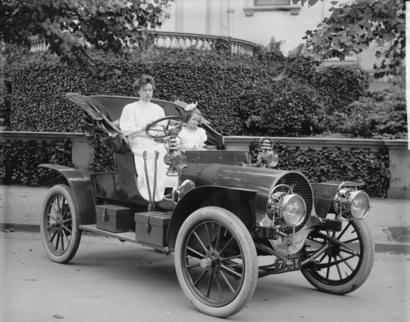
\includegraphics[width=\linewidth]{sample-franklin}
  \caption{1907 Franklin Model D roadster. Photograph by Harris \&
    Ewing, Inc. [Public domain], via Wikimedia
    Commons. (\url{https://goo.gl/VLCRBB}).}
  \Description{The 1907 Franklin Model D roadster.}
\end{figure}

\subsection{Data preprocessing}
In our experiments, we use the data parsed by SocialWays directly. For the ETH dataset, the parsing process can be illustrated by the Social Ways project, and for the UCY dataset, the parsing process is currently not included in the project and is not publicly available. But the parsed data is provided by Social Ways and is available for public download~\footnote{\url{http://www.dropbox.com/sh/lh1s41d1pqp8cbx/AAD4sB1JAiZIkCL7LHht-S4Ca}}.